%%%%%%%%%%%%%%%%%%%%%%%%%%%%%%%%%%%%%%%%%
% fphw Assignment
% LaTeX Template
% Version 1.0 (27/04/2019)
%
% This template originates from:
% https://www.LaTeXTemplates.com
%
% Authors:
% Class by Felipe Portales-Oliva (f.portales.oliva@gmail.com) with template 
% content and modifications by Vel (vel@LaTeXTemplates.com)
%
% Template (this file) License:
% CC BY-NC-SA 3.0 (http://creativecommons.org/licenses/by-nc-sa/3.0/)
%
%%%%%%%%%%%%%%%%%%%%%%%%%%%%%%%%%%%%%%%%%

%----------------------------------------------------------------------------------------
%	PACKAGES AND OTHER DOCUMENT CONFIGURATIONS
%----------------------------------------------------------------------------------------

\documentclass[
	12pt, % Default font size, values between 10pt-12pt are allowed
	%letterpaper, % Uncomment for US letter paper size
	%spanish, % Uncomment for Spanish
]{fphw}

% Template-specific packages
\usepackage[utf8]{inputenc} % Required for inputting international characters
\usepackage[T1]{fontenc} % Output font encoding for international characters
\usepackage{mathpazo} % Use the Palatino font

\usepackage{graphicx} % Required for including images

\usepackage{booktabs} % Required for better horizontal rules in tables

\usepackage{listings} % Required for insertion of code

\usepackage{enumerate} % To modify the enumerate environment

%\usepackage{caption}
%\usepackage{subcaption}

\usepackage[russian]{babel}

%----------------------------------------------------------------------------------------
%	ASSIGNMENT INFORMATION
%----------------------------------------------------------------------------------------

\title{Forensics Analysis Report} % Assignment title

\author{Russian Tea Room} % Student name

\date{October 31\textsuperscript{st}, 2020} % Due date

\institute{Computer Forensic Reference Data Sets (CFReDS)} % Institute or school name

\class{Ramy Chemak} % Course or class name

%\professor{Gustav Sicher} % Professor or teacher in charge of the assignment

%----------------------------------------------------------------------------------------

\begin{document}

\maketitle % Output the assignment title, created automatically using the information in the custom commands above

%----------------------------------------------------------------------------------------
%	ASSIGNMENT CONTENT
%----------------------------------------------------------------------------------------


\paragraph{}
\section*{Introduction}
\label{sec:intro}

\paragraph{}
This report describes the followed process to solve the “Russian Tea Room” case. Not all extracted information is useful for the main task (recover the stolen menu). This is a practice, so the other forensic-related skills, such as VBR reading or MPT recovery, might be put into practice despite being pointless to the case itself. The purpose is to use the disk as learning material and practice at best possible.\\


%\paragraph{}
\section{Disk pre-analysis}
\label{sec:docs}

I first notice that the MBR is probably broken. The data explicitly displays the error of an \textit{“Invalid
partition table”}. The MBR sector could easily be identified as it occupies the first 512b of the disk
(sector 0), ending with the signature \textit{55 AA}.

\begin{center}
	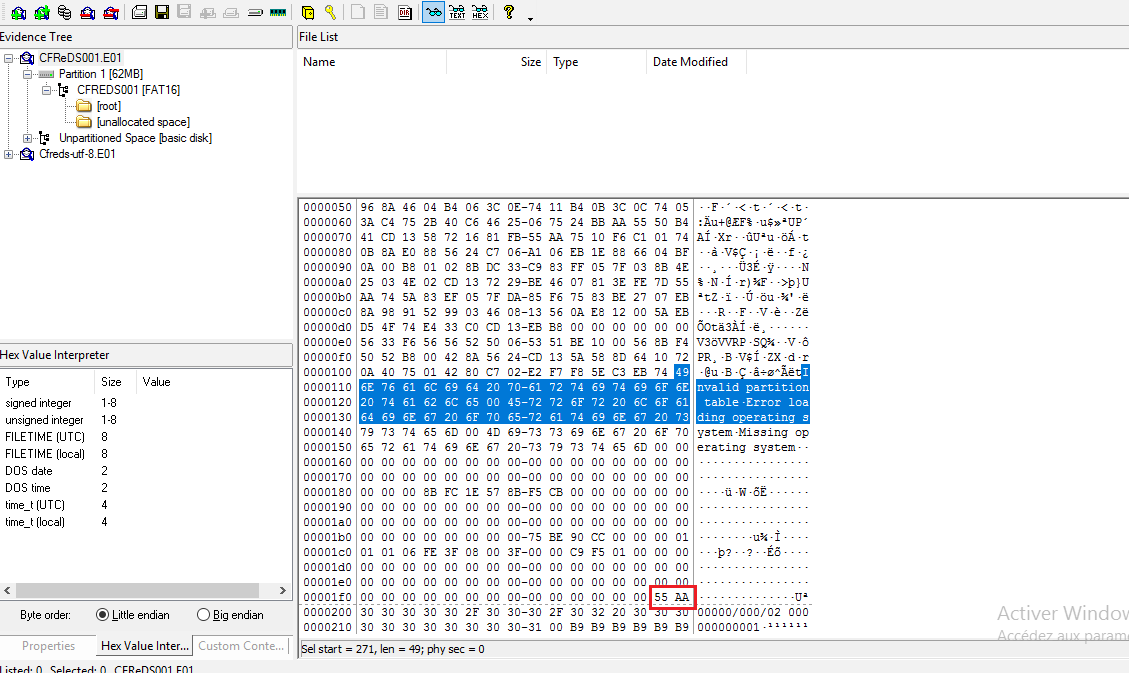
\includegraphics[width=0.9\columnwidth]{fig1.png}
	%\caption{\\\textit{Figure -1-}}
	\label{fig:fig1}
\end{center}
\vspace{2mm}

The MPT has one entry indicating the presence of only one partition. The byte 0x06 located at the
offset \textit{0x1c2} indicates that the file system we’re dealing with is a FAT16 (as FTK Imager has already
told). We therefore deduce the following information about the partition:

\begin{itemize}
	\item File system: FAT16
	\item CHS of partition end: 540 670
	\item LBA of start sector: 16 128
	\item Partition length: 128 457 sectors\\
\end{itemize}

The GPT partition was overwritten with 0xB9 (like much of the disk). There isn’t much to get from
anyway.\\

While considering the main task of this case, the information we have collected about the disk should
do the job. The task consists in recovering some information about a menu, probably lost somewhere
in a file. The start and size of partition tells us where we should be looking, and the file system will
guide us how to read, recover and carve eventual files.\\

We also have the volume boot record (VBR) for FAT16, from which we can extract a number of
information.

\begin{center}
	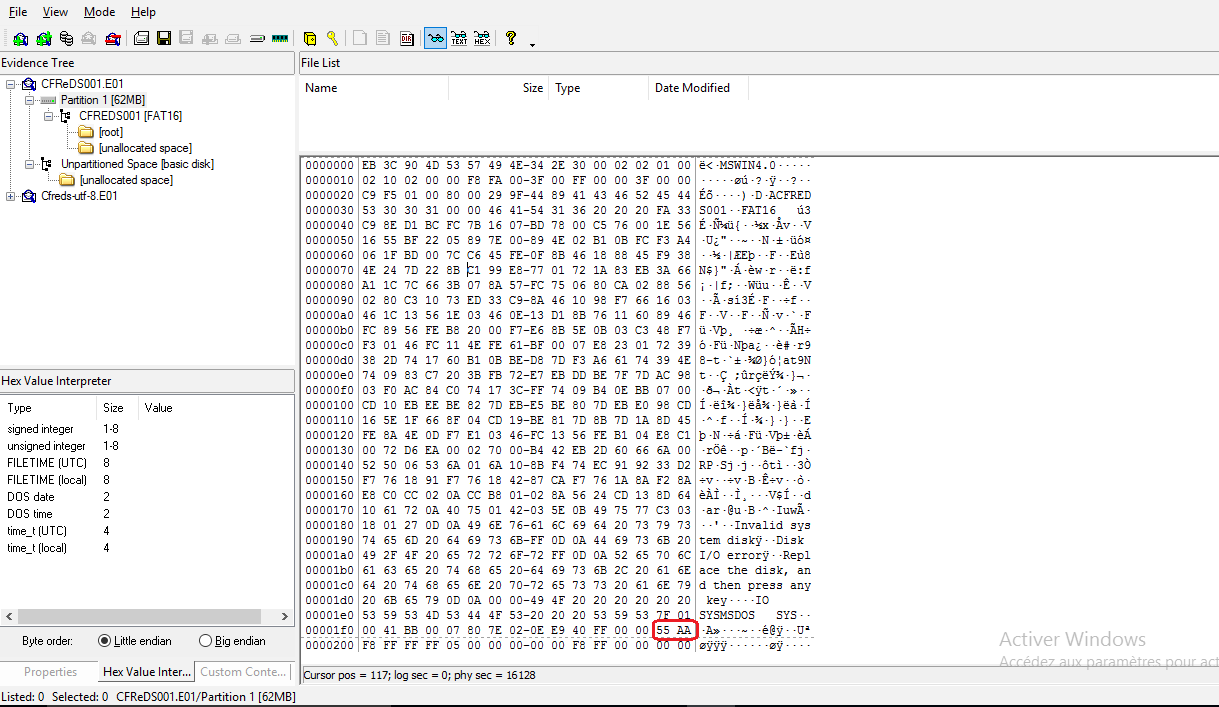
\includegraphics[width=0.9\columnwidth]{fig2.png}
	%\caption{\\\textit{Figure -1-}}
	\label{fig:fig2}
\end{center}
\vspace{2mm}

We can get the following information:

\begin{itemize}
	\item OEM ID:
	\item Sector size: 512b
	\item N° of sectors per cluster: 2
	\item Volume label: CFREDS001
	\item File system: FAT16
\end{itemize}

%\paragraph{}
\section{Data recovery}
\label{sec:doc1}

\paragraph{}
I first start a simple string search. I noticed that one of the text files found the file system contains
the beverages, which is one of the menu sections to recover. So I would guess that looking for the
string ‘Beverages’ might be a good lead to find something about the rest (a corrupt file to carve for
example).

\begin{center}
	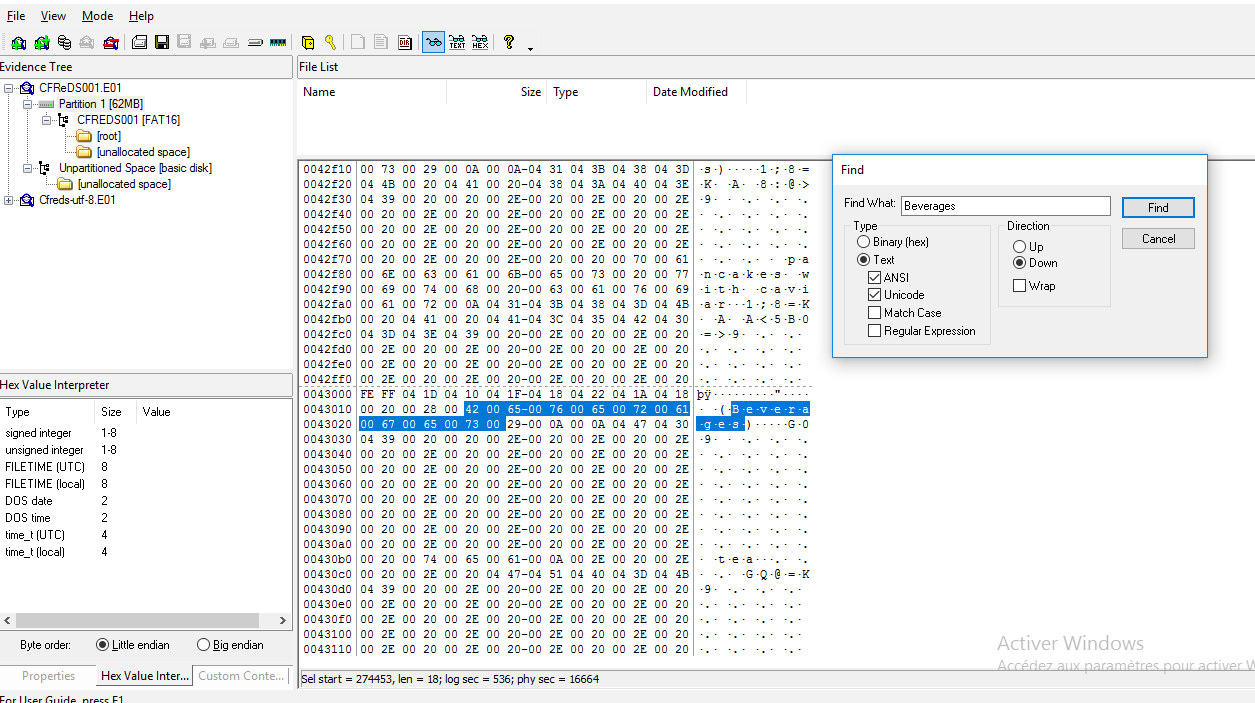
\includegraphics[width=0.9\columnwidth]{fig3.png}
	%\caption{\\\textit{Figure -1-}}
	\label{fig:fig3}
\end{center}
\vspace{2mm}

I go up until I reach the beginning of this written (cluster 16662). In short, I find what looks like the
start of the ‘Appetizers’ section, while all (or at least a big deal) of what is preceding it is empty.
According to instructions, the ‘Appetizers’ section is the first of menu sections to recover. So I may be
looking at the right cluster.\\

\begin{center}
	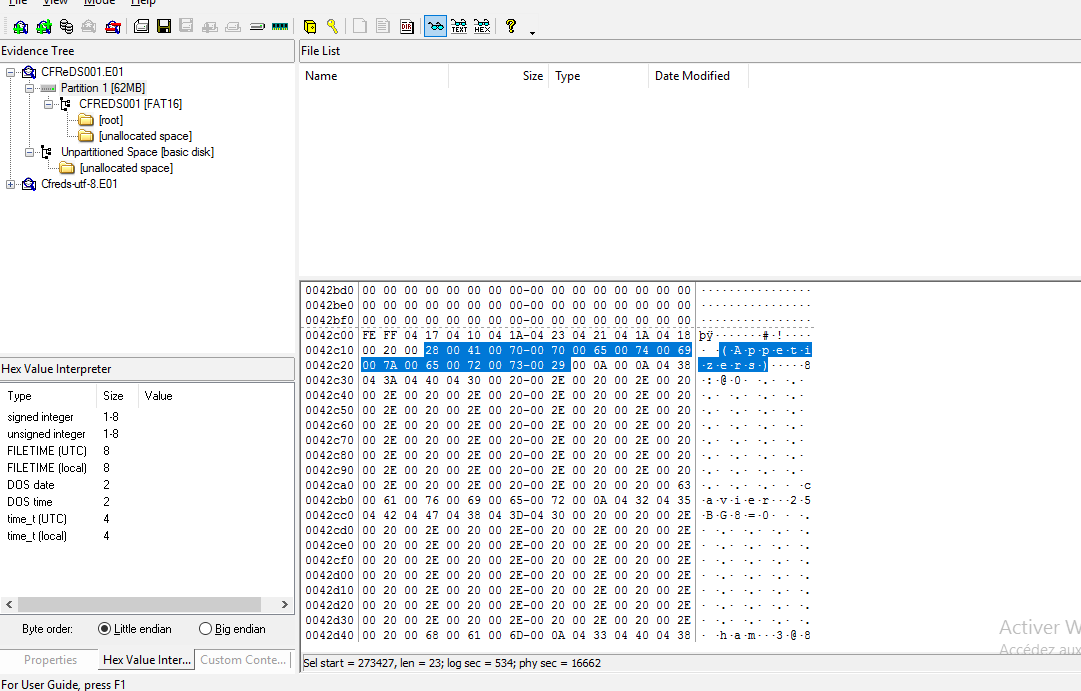
\includegraphics[width=0.9\columnwidth]{fig4.png}
	%\caption{\\\textit{Figure -1-}}
	\label{fig:fig4}
\end{center}
\vspace{2mm}

On cluster 16629, I could find several FAT16 file entries. By checking out the file attribute type (12\textsuperscript{th}
byte) in each record, we come to the following observations.\\

The first entry corresponds to the volume label, which is totally expectable. The four next entries
however correspond to four deleted files, with the first byte set to 0xE5. One of them is a read-only
hidden system volume and two are archive files. A last entry corresponds to an undeleted file
app.txt, which has already been recovered by FTK Imager. The file contains a portion of the menu to
recover.

\begin{center}
	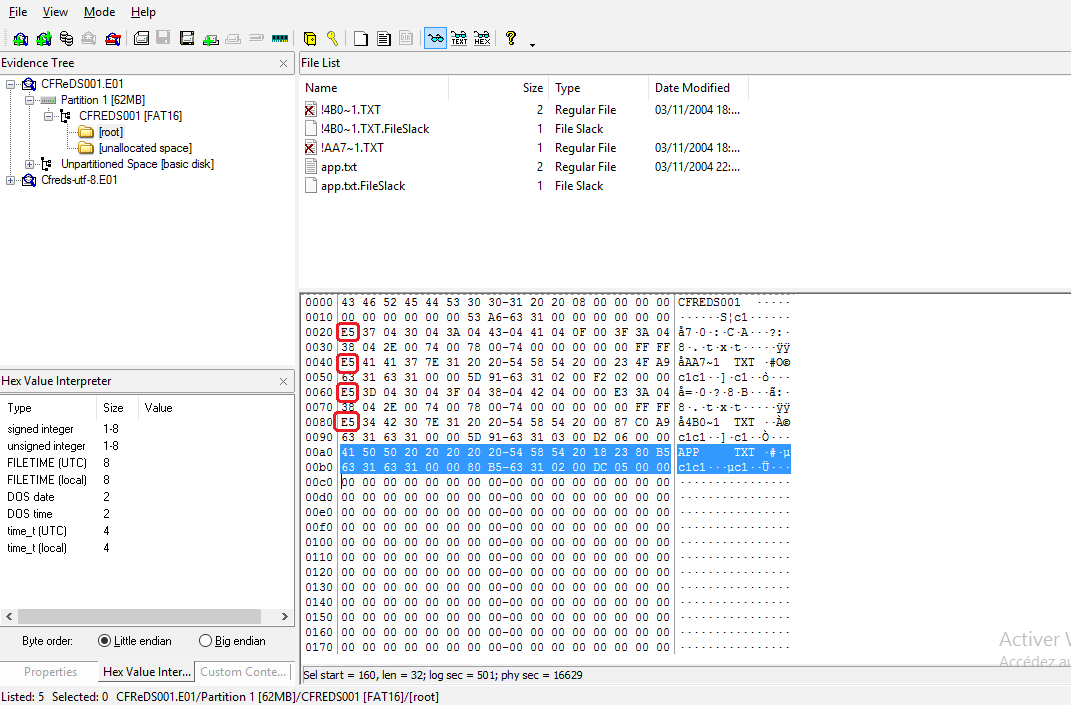
\includegraphics[width=0.8\columnwidth]{fig5.png}
	%\caption{\\\textit{Figure -1-}}
	\label{fig:fig5}
\end{center}
\vspace{2mm}

Two of those deleted files are of size 0 while two others have some weight. So I would deduce that
they might be worth looking into. Indeed, we are able to find some raw information in there, which
occurs to be helpful for further data reconstruction.

\begin{center}
	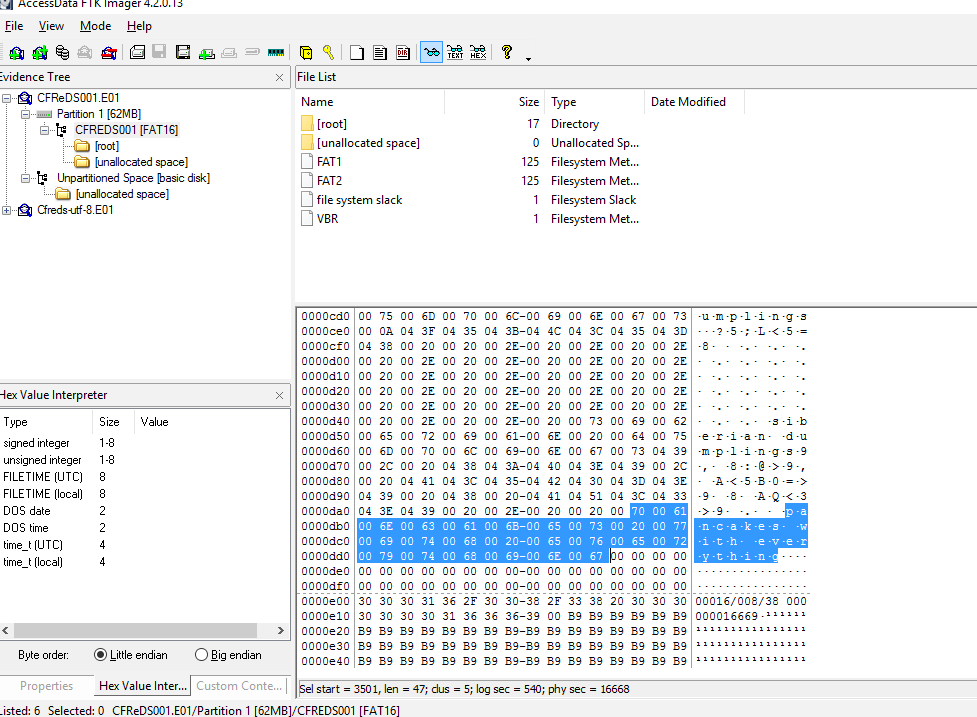
\includegraphics[width=0.8\columnwidth]{fig6.png}
	%\caption{\\\textit{Figure -1-}}
	\label{fig:fig6}
\end{center}
\vspace{2mm}

I end up with some overlapping parts between sections “Pancakes” and “Meat pies and dumplings”.
That’s odd and might suggest that I’ve made a mistake somewhere.\\

At this point, I was so far able to recover much of the stolen menu. But I still lack at least four
sections, which are: “Soup”, “Meat and Fish”, “Cheese and milk products” and “Dessert”. The first
partition doesn’t really provide further information. The rest of the disk is completely overwritten
either by \textit{0xB9} or just \textit{0x00}. The unpartitioned space remains so far undiscovered though. So I might be looking for a lead from there. I can’t really find anything concrete. Therefore, my last resort is the
classical string search. This way, I’m able to find some lost portions of text, all over the disk, which
allows me to reconstruct the rest of the stolen menu.

%\paragraph{}
\section{Recovered menu}
\label{sec:doc2}

\textbf{Appetizers - \foreignlanguage{russian}{ЗАКУСКИ}}

\begin{itemize}
	\item Cavier (probably caviar) - \foreignlanguage{russian}{икра}
	\item Ham - \foreignlanguage{russian}{ветчина}
	\item Mushrooms - \foreignlanguage{russian}{грибы}
	\item Sausage - \foreignlanguage{russian}{колбаса}
	\item Herring - \foreignlanguage{russian}{селёдка}
\end{itemize}

\textbf{Soup - \foreignlanguage{russian}{СУП}}

\begin{itemize}
	\item Borscht - \foreignlanguage{russian}{борщ}
	\item Cabbage soup
	\item Uzbek mutton soup
	\item Georgian mutton soup
	\item Fish soup
	\item Chicken soup
\end{itemize}

\textbf{Pancakes - \foreignlanguage{russian}{БЛИНЫ}:}

\begin{itemize}
	\item Pancakes with caviar - \foreignlanguage{russian}{блины с икрой}
	\item Stuffed buns - \foreignlanguage{russian}{блины с сметаной}
	\item Cheese dumplings - \foreignlanguage{russian}{вареники}
	\item Siberian dumplings – \foreignlanguage{russian}{пельмени}
	\item Pancakes with everything
\end{itemize}

\textbf{Meat pies and dumplings:}

\begin{itemize}
	\item Meat pie
	\item Stuffed buns- \foreignlanguage{russian}{блины с сметаной}
	\item Cheese dumplings- \foreignlanguage{russian}{вареники}
	\item Siberian dumplings – \foreignlanguage{russian}{пельмени}
\end{itemize}

\textbf{Meat and fish - \foreignlanguage{russian}{МЯСО И РЫБА}:}

\begin{itemize}
	\item Beef stroganoff
	\item Steak
	\item Cutlets
	\item Roast beef
	\item Chicken
	\item Duck
	\item Goose
	\item Pheasant
	\item Carp
	\item Herring
	\item Salomon
\end{itemize}

\textbf{Cheese and milk products - \foreignlanguage{russian}{СЫР И МОЛОЧНЫЕ}:}

\begin{itemize}
	\item Sour cream
	\item Cream
	\item Ewe’s cheese
	\item Butter milk
	\item Fresh cheese
	\item Farmer’s cheese
\end{itemize}

\textbf{Beverages – \foreignlanguage{russian}{НАПИТКИ}:}

\begin{itemize}
	\item Tea – \foreignlanguage{russian}{чай}
	\begin{itemize}
		\item Black - \foreignlanguage{russian}{чёрный}
		\item With milk - \foreignlanguage{russian}{с молоком}
		\item With lemon - \foreignlanguage{russian}{с лимоном}
	\end{itemize}
	\item Iced tea - \foreignlanguage{russian}{чай солодом}
	\item Mineral water - \foreignlanguage{russian}{минеральная вода}
	\item Coffee - \foreignlanguage{russian}{кофе}
	\item Milk - \foreignlanguage{russian}{молоко}
	\item Cognac - \foreignlanguage{russian}{коньяк}
	\item Vodka - \foreignlanguage{russian}{водка}
	\item Beer - \foreignlanguage{russian}{пиво}
	\item Wine - \foreignlanguage{russian}{вино}
\end{itemize}

\textbf{Dessert – \foreignlanguage{russian}{СЛАДКОЕ}:}

\begin{itemize}
	\item Ice cream
	\item Vanilla
	\item Fruit
	\item Chocolate
	\item Tart
	\begin{itemize}
		\item With lemon - \foreignlanguage{russian}{с лимоном}
		\item With cheese
	\end{itemize}
\end{itemize}

%\paragraph{}
\section*{Conclusion}
\label{sec:conclusion}

\paragraph{}
This case was useful to practice, among other things, system forensics, file recoery and file carving.\\


\bibliographystyle{plain}
\bibliography{links}

%----------------------------------------------------------------------------------------

\end{document}
